\documentclass[border={0.5cm 0.5cm 0.5cm 0.5cm}]{standalone}

\usepackage{tikz}
\usetikzlibrary{decorations.pathreplacing}	%for brackets

%Power and Perception Model
%Karrass, Chester. (1970). The Negotiating Game. New York: Thomas Y. Crownwell, p. 65

\begin{document}
	
	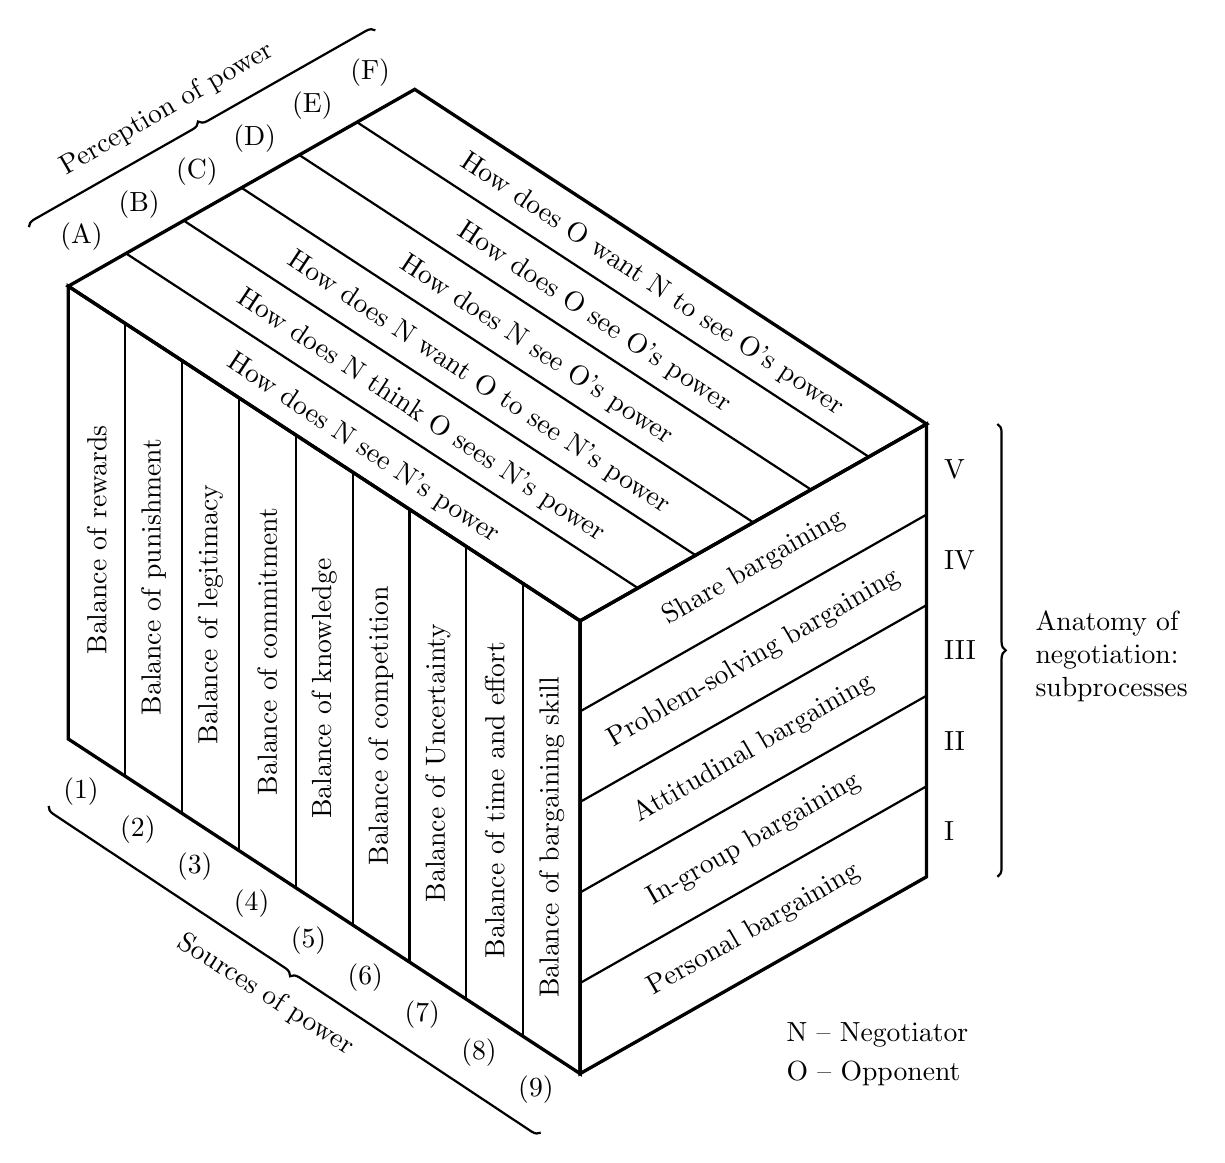
\begin{tikzpicture}
	%BOX
	\draw[very thick] (0,0)--(4.4,2.5)--(4.4,-3.25)--(0,-5.75)--cycle;		%bottom-right
	\draw[very thick] (0,0)--(-6.5,4.25)--(-6.5,-1.5)--(0,-5.75)--cycle;	%bottom-left
	\draw[very thick] (0,0)--(-6.5,4.25)--(-2.1,6.75)--(4.4,2.5)--cycle;	%top
	
	%lines
	\foreach \x in {1,...,5}{
	\draw[thick] (0,0-\x*1.15)--(4.4,2.5-\x*1.15);						%bottom-right
	\draw[thick] (4.4/6*\x,2.5/6*\x)--(-6.5+4.4/6*\x,4.25+2.5/6*\x);	%top
		}
	\foreach \x in {1,...,9}
	\draw[thick] (-6.5/9*\x,4.25/9*\x)--(-6.5/9*\x,-5.75+4.25/9*\x);	%bottom-left
	
	%LABELS -- BOTTOM-RIGHT
	\foreach \x/\n [count=\i] in {{Personal bargaining}/{I},{In-group bargaining}/{II},{Attitudinal bargaining}/{III},{Problem-solving bargaining}/{IV},{Share bargaining}/{V}}{
	\node at (2.20,-4.5-1.15/2+1.15*\i) {\rotatebox{30}{\x}};
	\node[align=left,right] at (4.5,-3.825+1.15*\i) {\n};
	}
	\draw[decorate,decoration={brace,amplitude=3pt},thick] (5.3,2.5)--(5.3,-3.25);
	\node[align=left] at (6.75,-0.45) {Anatomy of\\negotiation:\\subprocesses};
	
	%LABELS -- BOTTOM-LEFT (NB: goes left-to-right)
	\foreach \x [count=\i] in {{Balance of rewards},{Balance of punishment},{Balance of legitimacy},{Balance of commitment},{Balance of knowledge},{Balance of competition},{Balance of Uncertainty},{Balance of time and effort},{Balance of bargaining skill}}{
		\node at (-6.5-6.5/9/2+6.5/9*\i,1.5-4.25/9*\i)  {\rotatebox{90}{\x}};
		\node at (-6.7-6.5/9/2+6.5/9*\i,-1.7-4.25/9*\i) {(\i)};
	}
	\draw[decorate,decoration={brace,amplitude=3pt},thick] (-0.5,-6.5)--(-6.75,-2.35);
	\node at (-4,-4.75)  {\rotatebox{-32.5}{Sources of power}};
	
	%LABELS -- TOP
	\foreach \x/\n [count=\i] in {{How does N see N's power}/{A},{How does N think O sees N's power}/{B},{How does N want O to see N's power}/{C},{How does N see O's power}/{D},{How does O see O's power}/{E},{How does O want N to see O's power}/{F}}{
	\node at (-6.25/2-4.4/6/2+4.4/6*\i,4.25/2-4.25/6/2+2.5/6*\i) {\rotatebox{-33.5}{\x}};
	\node at (-6.7-4.4/6/2+4.4/6*\i,4.25+2.5/6/2+2.5/6*\i) {(\n)};
	}
	\draw[decorate,decoration={brace,amplitude=3pt},thick] (-6.5-0.5,4.25+0.75)--(-2.1-0.5,6.75+0.75);
	\node at (-5.25,6.5)  {\rotatebox{30}{Perception of power}};
	
	%LABELS -- LEGEND
	\node[align=left,right] at (2.5,-5.25)  {N -- Negotiator};
	\node[align=left,right] at (2.5,-5.75)  {O -- Opponent};
	
	\end{tikzpicture}
	
\end{document}